%%%%%%%%%%%%%%%%%%%%%%%%%%%%%%%%%%%%%%%%%
% Beamer Presentation
% LaTeX Template
% Version 2.0 (March 8, 2022)
%
% This template originates from:
% https://www.LaTeXTemplates.com
%
% Author:
% Vel (vel@latextemplates.com)
%
% License:
% CC BY-NC-SA 4.0 (https://creativecommons.org/licenses/by-nc-sa/4.0/)
%
%%%%%%%%%%%%%%%%%%%%%%%%%%%%%%%%%%%%%%%%%

%----------------------------------------------------------------------------------------
%	PACKAGES AND OTHER DOCUMENT CONFIGURATIONS
%----------------------------------------------------------------------------------------

\documentclass[
11pt, % Set the default font size, options include: 8pt, 9pt, 10pt, 11pt, 12pt, 14pt, 17pt, 20pt
%t, % Uncomment to vertically align all slide content to the top of the slide, rather than the default centered
%aspectratio=169, % Uncomment to set the aspect ratio to a 16:9 ratio which matches the aspect ratio of 1080p and 4K screens and projectors
]{beamer}

\graphicspath{{Images/}{./}} % Specifies where to look for included images (trailing slash required)

\usepackage{booktabs} % Allows the use of \toprule, \midrule and \bottomrule for better rules in tables

%---Inicio cosas matematicas---
\usepackage{tikz}
\usetikzlibrary{positioning}
\usetikzlibrary{shadows} %shadedbox

%---Fin cosas matematicas---


%----------------------------------------------------------------------------------------
%	SELECT LAYOUT THEME
%----------------------------------------------------------------------------------------

% Beamer comes with a number of default layout themes which change the colors and layouts of slides. Below is a list of all themes available, uncomment each in turn to see what they look like.

%\usetheme{default}
%\usetheme{AnnArbor}
%\usetheme{Antibes}
%\usetheme{Bergen}
%\usetheme{Berkeley}
%\usetheme{Berlin}
%\usetheme{Boadilla}
%\usetheme{CambridgeUS}
%\usetheme{Copenhagen}
%\usetheme{Darmstadt}
%\usetheme{Dresden}
%\usetheme{Frankfurt}
%\usetheme{Goettingen}
%\usetheme{Hannover}
%\usetheme{Ilmenau}
%\usetheme{JuanLesPins}
%\usetheme{Luebeck}
\usetheme{Madrid}
%\usetheme{Malmoe}
%\usetheme{Marburg}
%\usetheme{Montpellier}
%\usetheme{PaloAlto}
%\usetheme{Pittsburgh}
%\usetheme{Rochester}
%\usetheme{Singapore}
%\usetheme{Szeged}
%\usetheme{Warsaw}

%----------------------------------------------------------------------------------------
%	SELECT COLOR THEME
%----------------------------------------------------------------------------------------

% Beamer comes with a number of color themes that can be applied to any layout theme to change its colors. Uncomment each of these in turn to see how they change the colors of your selected layout theme.

%\usecolortheme{albatross}
%\usecolortheme{beaver}
%\usecolortheme{beetle}
%\usecolortheme{crane}
%\usecolortheme{dolphin}
%\usecolortheme{dove}
%\usecolortheme{fly}
%\usecolortheme{lily}
%\usecolortheme{monarca}
%\usecolortheme{seagull}
%\usecolortheme{seahorse}
%\usecolortheme{spruce}
%\usecolortheme{whale}
%\usecolortheme{wolverine}

%----------------------------------------------------------------------------------------
%	SELECT FONT THEME & FONTS
%----------------------------------------------------------------------------------------

% Beamer comes with several font themes to easily change the fonts used in various parts of the presentation. Review the comments beside each one to decide if you would like to use it. Note that additional options can be specified for several of these font themes, consult the beamer documentation for more information.

\usefonttheme{default} % Typeset using the default sans serif font
%\usefonttheme{serif} % Typeset using the default serif font (make sure a sans font isn't being set as the default font if you use this option!)
%\usefonttheme{structurebold} % Typeset important structure text (titles, headlines, footlines, sidebar, etc) in bold
%\usefonttheme{structureitalicserif} % Typeset important structure text (titles, headlines, footlines, sidebar, etc) in italic serif
%\usefonttheme{structuresmallcapsserif} % Typeset important structure text (titles, headlines, footlines, sidebar, etc) in small caps serif

%------------------------------------------------

%\usepackage{mathptmx} % Use the Times font for serif text
\usepackage{palatino} % Use the Palatino font for serif text

%\usepackage{helvet} % Use the Helvetica font for sans serif text
\usepackage[default]{opensans} % Use the Open Sans font for sans serif text
%\usepackage[default]{FiraSans} % Use the Fira Sans font for sans serif text
%\usepackage[default]{lato} % Use the Lato font for sans serif text

%----------------------------------------------------------------------------------------
%	SELECT INNER THEME
%----------------------------------------------------------------------------------------

% Inner themes change the styling of internal slide elements, for example: bullet points, blocks, bibliography entries, title pages, theorems, etc. Uncomment each theme in turn to see what changes it makes to your presentation.

%\useinnertheme{default}
\useinnertheme{circles}
%\useinnertheme{rectangles}
%\useinnertheme{rounded}
%\useinnertheme{inmargin}

%----------------------------------------------------------------------------------------
%	SELECT OUTER THEME
%----------------------------------------------------------------------------------------

% Outer themes change the overall layout of slides, such as: header and footer lines, sidebars and slide titles. Uncomment each theme in turn to see what changes it makes to your presentation.

%\useoutertheme{default}
%\useoutertheme{infolines}
%\useoutertheme{miniframes}
%\useoutertheme{smoothbars}
%\useoutertheme{sidebar}
%\useoutertheme{split}
%\useoutertheme{shadow}
%\useoutertheme{tree}
%\useoutertheme{smoothtree}

%\setbeamertemplate{footline} % Uncomment this line to remove the footer line in all slides
%\setbeamertemplate{footline}[page number] % Uncomment this line to replace the footer line in all slides with a simple slide count

%\setbeamertemplate{navigation symbols}{} % Uncomment this line to remove the navigation symbols from the bottom of all slides

%----------------------------------------------------------------------------------------
%	PRESENTATION INFORMATION
%----------------------------------------------------------------------------------------

\title[Laboratorio de Modelaci\'on]{MAT282 - Laboratorio de Modelaci\'on I} % The short title in the optional parameter appears at the bottom of every slide, the full title in the main parameter is only on the title page

\subtitle{Optimization and visualization of the planning of a three-node electrical network during a day} % Presentation subtitle, remove this command if a subtitle isn't required

\author[Vicente Moreno \and Martina Blanco]{Vicente Moreno \and Martina Blanco \\ Specialist: Nicol\'as Hern\'andez} % Presenter name(s), the optional parameter can contain a shortened version to appear on the bottom of every slide, while the main parameter will appear on the title slide

\institute[USM]{Universidad T\'ecnica Federico Santa Mar\'ia \\ vicente.moreno@usm.cl \\ martina.blanco@usm.cl} % Your institution, the optional parameter can be used for the institution shorthand and will appear on the bottom of every slide after author names, while the required parameter is used on the title slide and can include your email address or additional information on separate lines

\date[\today]{\today} % Presentation date or conference/meeting name, the optional parameter can contain a shortened version to appear on the bottom of every slide, while the required parameter value is output to the title slide

%----------------------------------------------------------------------------------------

\begin{document}
	
	%----------------------------------------------------------------------------------------
	%	TITLE SLIDE
	%----------------------------------------------------------------------------------------
	
	\begin{frame}
		\titlepage % Output the title slide, automatically created using the text entered in the PRESENTATION INFORMATION block above
	\end{frame}
	
	%----------------------------------------------------------------------------------------
	%	TABLE OF CONTENTS SLIDE
	%----------------------------------------------------------------------------------------
	
	% The table of contents outputs the sections and subsections that appear in your presentation, specified with the standard \section and \subsection commands. You may either display all sections and subsections on one slide with \tableofcontents, or display each section at a time on subsequent slides with \tableofcontents[pausesections]. The latter is useful if you want to step through each section and mention what you will discuss.
	
	\begin{frame}
		\frametitle{Presentation Overview} % Slide title, remove this command for no title
		
		\tableofcontents % Output the table of contents (all sections on one slide)
		%\tableofcontents[pausesections] % Output the table of contents (break sections up across separate slides)
	\end{frame}
	
	%----------------------------------------------------------------------------------------
	%	PRESENTATION BODY SLIDES
	%----------------------------------------------------------------------------------------
	
	\section{Introduction}
	\begin{frame}
		\frametitle{Introduction}
		\begin{itemize}
			\item The main objective of our work is to model the Chilean electrical network throughout a day, to obtain a planning to be carried out to satisfy the demands at the lowest possible cost.
			\item To achieve the objective, we developed a code in Python that solves this problem and provides relevant information for the optimal planning of the network during a day through data and graphs.
		\end{itemize}
	\end{frame}
	
	\begin{frame}
		\frametitle{A graph of the chilean electricity network}
		\begin{itemize}
			\item We can model the chilean electricity network as a directed connected graph.
		\end{itemize}
		
		\begin{center}
			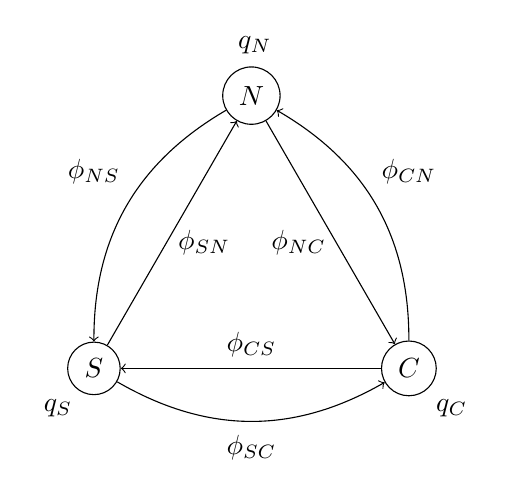
\begin{tikzpicture}
				
				\node[circle,draw] (N) at (2,3.4641) {$N$};
				\node[circle,draw] (S) at (0,0) {$S$};
				\node[circle,draw] (C) at (4,0) {$C$};
				
				\draw[->] (N) -- (C);
				\draw[->] (C) to[bend right] (N);
				\draw[->] (C) -- (S);
				\draw[->] (S) to[bend right] (C);
				\draw[->] (S) -- (N);
				\draw[->] (N) to[bend right] (S);
				
				\node (QS) at (-0.5,-0.5) {\(\ q_S\)} ;
				\node (QC) at (4.5,-0.5) {\(\ q_C\)} ;
				\node (QN) at (2,4.1) {\(\ q_N\)} ;
				
				\node (SN) at (1.4,1.6) {\(\phi_{\text{SN}}\)} ;
				\node (NC) at (2.6,1.6) {\(\phi_{\text{NC}}\)} ;
				\node (CS) at (2,0.3) {\(\phi_{\text{CS}}\)} ;
				\node (NS) at (0,2.5) {\(\phi_{\text{NS}}\)} ;
				\node (CN) at (4,2.5) {\(\phi_{\text{CN}}\)} ;
				\node (SC) at (2,-1) {\(\phi_{\text{SC}}\)} ;
				
			\end{tikzpicture} \\
		\end{center}
	\end{frame}
	
	
	%------------------------------------------------
	
	\section{Theory}
	
	\begin{frame}
		\frametitle{General form of the electrical network problem}
		
		\begin{equation*}\begin{aligned}
				\min_{(q,\phi)} \quad & \sum_{i\in I}\operatorname{p}_i(q_i) \\
				\textrm{s.a.} \quad & q_i+\sum_{e\in E_i}\left(\phi_e-\operatorname{r}(\phi_e)\right)-\sum_{s\in S_i}\phi_s=D_i, & & \forall i \in I \\
				& q_i\in[0,Q_i], & & \forall i \in I \\
				& \phi_j\geq0, & & \forall j \in E
		\end{aligned}\end{equation*}
	\end{frame}
	
	%------------------------------------------------
	
	\begin{frame}
		\frametitle{Main equation to solve}

		\begin{equation*}\begin{aligned}
				\min_{(q,\phi)} \quad & \operatorname{p}_N(q_N)+\operatorname{p}_S(q_S)+\operatorname{p}_C(q_C) \\
				\textrm{s.a.} \quad & q_N+(1-r)(\phi_{SN}+\phi_{CN})-(\phi_{NS}+\phi_{NC})=D_N, \\
				\quad & q_S+(1-r)(\phi_{NS}+\phi_{CS})-(\phi_{SN}+\phi_{SC})=D_S, \\
				\quad & q_C+(1-r)(\phi_{SC}+\phi_{NC})-(\phi_{CS}+\phi_{CN})=D_C, \\
				& q_N\in[0,Q_N], \\
				& q_S\in[0,Q_S], \\
				& q_C\in[0,Q_C], \\
				& \phi_{NS},\phi_{SN},\phi_{SC},\phi_{CS},\phi_{NC},\phi_{CN}\geq0.
		\end{aligned}\end{equation*}
	\end{frame}
	
	%------------------------------------------------
	
	\section{Mathematical analysis for solutions}
	\begin{frame}
		\frametitle{Feasible Solutions v/s Optimal Solutions}
		
		\begin{itemize}
			\item The function to optimize only depends on the electricity production variables.
			\item If A and B are two feasible solutions such that \(q_i^A\leq q_i^B,\,\forall i \in I\), then B cannot be an optimal solution.
		\end{itemize}
		
	\end{frame}
	
	%------------------------------------------------
	
	\subsection{Mutual flux}
	\begin{frame}
		\frametitle{Mutual flux}
		
		\begin{itemize}
			\item South and Center nodes are using both directional fluxes at the same time (net energy loss).
			\item Lowest flux can be subtracted to both fluxes.
		\end{itemize}
		
			\begin{center}
			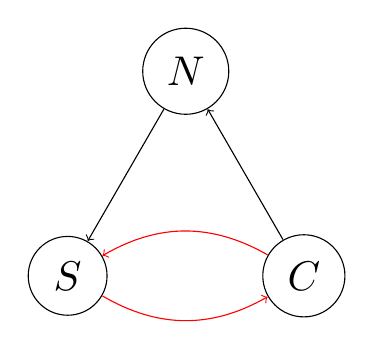
\begin{tikzpicture}[scale=1.5, every node/.style={scale=1.5}]
				\node[circle,draw] (N1) at (1,1.732) {$N$};
				\node[circle,draw] (S1) at (0,0) {$S$};
				\node[circle,draw] (C1) at (2,0) {$C$};
				
				\draw[->] (C1) -- (N1);
				\draw[->] (N1) -- (S1);
				\draw[red,->] (S1) to[bend right] (C1);
				\draw[red,->] (C1) to[bend right] (S1);
			\end{tikzpicture}
			\end{center}
	\end{frame}
	
	%------------------------------------------------
	
	\begin{frame}
		\frametitle{Remaining graphs}
			\begin{center}
			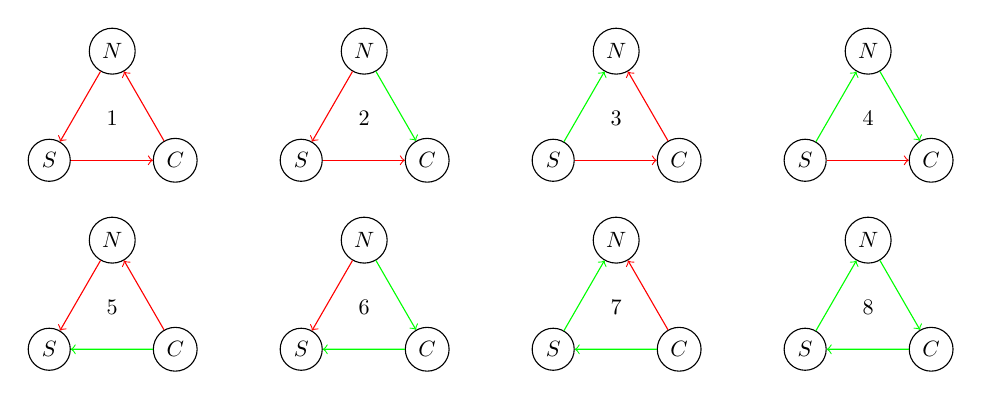
\begin{tikzpicture}[scale=0.8, every node/.style={scale=0.8}]
				
				\node (G1) at (1,0.66) {$1$};
				\node[circle,draw] (N1) at (1,1.732) {$N$};
				\node[circle,draw] (S1) at (0,0) {$S$};
				\node[circle,draw] (C1) at (2,0) {$C$};
				
				\draw[red,->] (C1) -- (N1);
				\draw[red,->] (N1) -- (S1);
				\draw[red,->] (S1) -- (C1);
				
				\node (G2) at (5,0.66) {$2$};
				\node[circle,draw] (N2) at (5,1.732) {$N$};
				\node[circle,draw] (S2) at (4,0) {$S$};
				\node[circle,draw] (C2) at (6,0) {$C$};
				
				\draw[green,->] (N2) -- (C2);
				\draw[red,->] (N2) -- (S2);
				\draw[red,->] (S2) -- (C2);
				
				\node (G3) at (9,0.66) {$3$};
				\node[circle,draw] (N3) at (9,1.732) {$N$};
				\node[circle,draw] (S3) at (8,0) {$S$};
				\node[circle,draw] (C3) at (10,0) {$C$};
				
				\draw[red,->] (C3) -- (N3);
				\draw[green,->] (S3) -- (N3);
				\draw[red,->] (S3) -- (C3);
				
				\node (G4) at (13,0.66) {$4$};
				\node[circle,draw] (N4) at (13,1.732) {$N$};
				\node[circle,draw] (S4) at (12,0) {$S$};
				\node[circle,draw] (C4) at (14,0) {$C$};
				
				\draw[green,->] (N4) -- (C4);
				\draw[green,->] (S4) -- (N4);
				\draw[red,->] (S4) -- (C4);
				
				\node (G5) at (1,-2.33) {$5$};
				\node[circle,draw] (N5) at (1,-1.268) {$N$};
				\node[circle,draw] (S5) at (0,-3) {$S$};
				\node[circle,draw] (C5) at (2,-3) {$C$};
				
				\draw[red,->] (C5) -- (N5);
				\draw[red,->] (N5) -- (S5);
				\draw[green,->] (C5) -- (S5);
				
				\node (G6) at (5,-2.33) {$6$};
				\node[circle,draw] (N6) at (5,-1.268) {$N$};
				\node[circle,draw] (S6) at (4,-3) {$S$};
				\node[circle,draw] (C6) at (6,-3) {$C$};
				
				\draw[green,->] (N6) -- (C6);
				\draw[red,->] (N6) -- (S6);
				\draw[green,->] (C6) -- (S6);
				
				\node (G7) at (9,-2.33) {$7$};
				\node[circle,draw] (N7) at (9,-1.268) {$N$};
				\node[circle,draw] (S7) at (8,-3) {$S$};
				\node[circle,draw] (C7) at (10,-3) {$C$};
				
				\draw[red,->] (C7) -- (N7);
				\draw[green,->] (S7) -- (N7);
				\draw[green,->] (C7) -- (S7);
				
				\node (G8) at (13,-2.33) {$8$};
				\node[circle,draw] (N8) at (13,-1.268) {$N$};
				\node[circle,draw] (S8) at (12,-3) {$S$};
				\node[circle,draw] (C8) at (14,-3) {$C$};
				
				\draw[green,->] (N8) -- (C8);
				\draw[green,->] (S8) -- (N8);
				\draw[green,->] (C8) -- (S8);
				
			\end{tikzpicture}
		\end{center}
	\end{frame}
	
	
	%------------------------------------------------
	\subsection{Graph similarity}
	\begin{frame}
		\frametitle{Graph symmetry}
	
		\begin{center}
			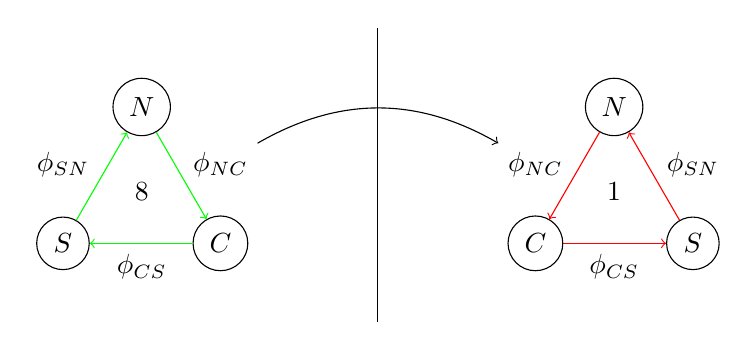
\begin{tikzpicture}
				
				\node (G8) at (1,0.66) {$8$};
				\node[circle,draw] (N8) at (1,1.732) {$N$};
				\node[circle,draw] (S8) at (0,0) {$S$};
				\node[circle,draw] (C8) at (2,0) {$C$};
				
				\node (f1) at (0,1) {$\phi_{SN}$};
				\node (f2) at (2,1) {$\phi_{NC}$};
				\node (f3) at (1,-0.3) {$\phi_{CS}$};
				
				\draw[green,->] (N8) -- (C8);
				\draw[green,->] (S8) -- (N8);
				\draw[green,->] (C8) -- (S8);
				
				\node (G1) at (7,0.66) {$1$};
				\node[circle,draw] (N1) at (7,1.732) {$N$};
				\node[circle,draw] (S1) at (6,0) {$C$};
				\node[circle,draw] (C1) at (8,0) {$S$};
				
				\node (f4) at (6,1) {$\phi_{NC}$};
				\node (f5) at (8,1) {$\phi_{SN}$};
				\node (f6) at (7,-0.3) {$\phi_{CS}$};
				
				\draw[red,->] (C1) -- (N1);
				\draw[red,->] (N1) -- (S1);
				\draw[red,->] (S1) -- (C1);
				
				\draw[->] (f2) to[bend left] (f4);
				\draw[-] (4,-1) to (4,2.732);
				
			\end{tikzpicture}
		\end{center}
		
		\begin{itemize}
			\item If an algorithm could solve Graph 1, we could solve Graph 8 via permutations of variables! (keep in mind...)
		\end{itemize}
	\end{frame}
	
	%------------------------------------------------
	
	\begin{frame}
		\frametitle{Splitting the problem}
		
		\small
		\begin{equation*}\begin{aligned}
				& \text{\hspace{1cm}Subproblem 1}& & \text{\hspace{1cm}Subproblem 2}  \\
				\min_{(q,\phi)} \quad & \operatorname{p}_N(q_N)+\operatorname{p}_S(q_S)+\operatorname{p}_C(q_C) & \min_{(q,\phi)} \quad & \operatorname{p}_N(q_N)+\operatorname{p}_S(q_S)+\operatorname{p}_C(q_C) \\
				\textrm{s.a.} \quad & q_N+(1-r)\phi_{CN}-\phi_{NS}=D_N & \textrm{s.a.} \quad & q_N-\phi_{NS}-\phi_{NC}=D_N \\
				& q_S+(1-r)\phi_{NS}-\phi_{SC}=D_S & & q_S+(1-r)\phi_{NS}-\phi_{SC}=D_S \\
				& q_C+(1-r)\phi_{SC}-\phi_{CN}=D_C & & q_C+(1-r)(\phi_{SC}+\phi_{NC})=D_C \\
				& q_N\in[0,Q_N] & & q_N\in[0,Q_N] \\
				& q_S\in[0,Q_S] & & q_S\in[0,Q_S] \\
				& q_C\in[0,Q_C] & & q_C\in[0,Q_C] \\
				& \phi_{NS},\phi_{SC},\phi_{CN}\geq0 & & \phi_{NS},\phi_{SC},\phi_{NC}\geq0 
		\end{aligned}\end{equation*}
		\normalsize
	\end{frame}
	
	%------------------------------------------------
	\subsection{Circular flux}
	\begin{frame}
		\frametitle{Subproblem 1 - Circular flux}
		\begin{itemize}
			\item Very similar to a Mutual Flux, but with a longer chain of fluxes (net energy loss on the whole chain).
			\item Lowest flux in the chain can be subtracted to all fluxes
		\end{itemize}
		
		\begin{center}
			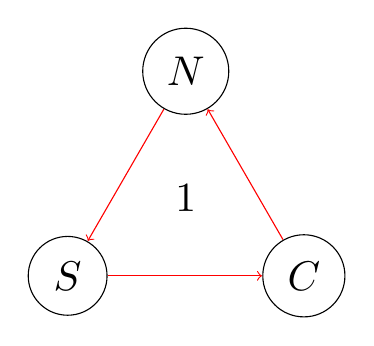
\begin{tikzpicture}[scale=1.5, every node/.style={scale=1.5}]
				\node (G1) at (1,0.66) {$1$};
				\node[circle,draw] (N1) at (1,1.732) {$N$};
				\node[circle,draw] (S1) at (0,0) {$S$};
				\node[circle,draw] (C1) at (2,0) {$C$};
				
				\draw[red,->] (C1) -- (N1);
				\draw[red,->] (N1) -- (S1);
				\draw[red,->] (S1) -- (C1);
			\end{tikzpicture}
		\end{center}
	\end{frame}
	
	%------------------------------------------------
	\begin{frame}
		\frametitle{Remaining graphs}
		\begin{center}
			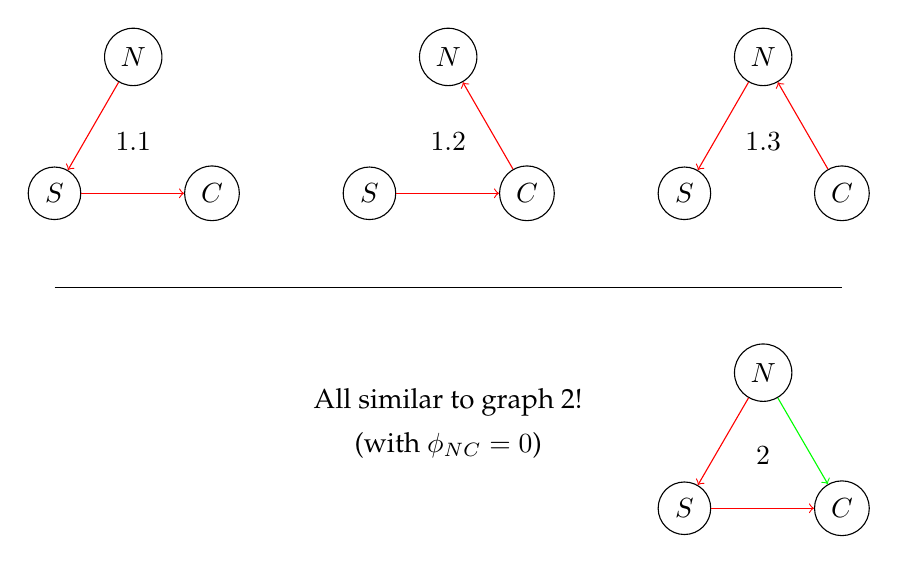
\begin{tikzpicture}
				
				\node (G1) at (1,0.66) {$1.1$};
				\node[circle,draw] (N1) at (1,1.732) {$N$};
				\node[circle,draw] (S1) at (0,0) {$S$};
				\node[circle,draw] (C1) at (2,0) {$C$};
				
				\draw[red,->] (S1) -- (C1);
				\draw[red,->] (N1) -- (S1);
				
				\node (G2) at (5,0.66) {$1.2$};
				\node[circle,draw] (N2) at (5,1.732) {$N$};
				\node[circle,draw] (S2) at (4,0) {$S$};
				\node[circle,draw] (C2) at (6,0) {$C$};
				
				\draw[red,->] (C2) -- (N2);
				\draw[red,->] (S2) -- (C2);
				
				\node (G3) at (9,0.66) {$1.3$};
				\node[circle,draw] (N3) at (9,1.732) {$N$};
				\node[circle,draw] (S3) at (8,0) {$S$};
				\node[circle,draw] (C3) at (10,0) {$C$};
				
				\draw[red,->] (N3) -- (S3);
				\draw[red,->] (C3) -- (N3);
				
				\draw (0,-1.2) -- (10,-1.2);
				
				\node (text) at (5,-2.66) {All similar to graph 2!};
				\node (text) at (5,-3.2) {(with \(\phi_{NC}=0\))};
				
				\node (G6) at (9,-3.33) {$2$};
				\node[circle,draw] (N6) at (9,-2.278) {$N$};
				\node[circle,draw] (S6) at (8,-4) {$S$};
				\node[circle,draw] (C6) at (10,-4) {$C$};
				
				\draw[red,->] (S6) -- (C6);
				\draw[red,->] (N6) -- (S6);
				\draw[green,->] (N6) -- (C6);
				
			\end{tikzpicture}
		\end{center}
		\begin{itemize}
			\item Subproblem 1 is \textbf{contained} in Subproblem 2.
		\end{itemize}
	\end{frame}
	
	%------------------------------------------------
	\subsection{Multiple routes}
	\begin{frame}
		\frametitle{Subproblem 2 - Multiple routes}
		
		\begin{itemize}
			\item There exist two routes to get from the North to Center node!
			\item Both \(\phi_{NS}\) and \(\phi_{SC}\) cannot be used at the same time
		\end{itemize}
		

		
		\begin{center}
			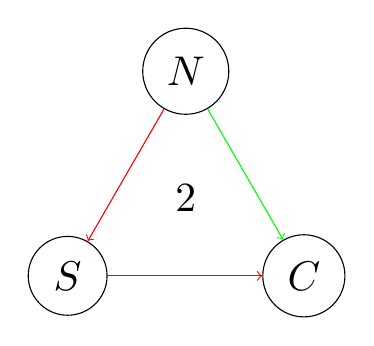
\begin{tikzpicture}[scale=1.5, every node/.style={scale=1.5}]
				\node (G2) at (5,0.66) {$2$};
				\node[circle,draw] (N2) at (5,1.732) {$N$};
				\node[circle,draw] (S2) at (4,0) {$S$};
				\node[circle,draw] (C2) at (6,0) {$C$};
				
				\draw[green,->] (N2) -- (C2);
				\draw[red,->] (N2) -- (S2);
				\draw[red,->] (S2) -- (C2);
			\end{tikzpicture}
		\end{center}
	\end{frame}
	
	
	%------------------------------------------------
	\begin{frame}
		\frametitle{Possible graphs after simplification}
		\begin{center}
			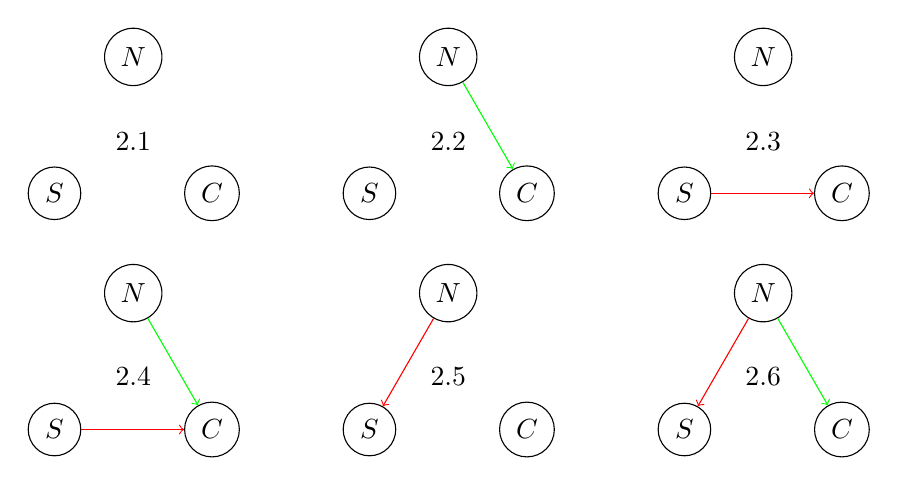
\begin{tikzpicture}
				
				\node (G1) at (1,0.66) {$2.1$};
				\node[circle,draw] (N1) at (1,1.732) {$N$};
				\node[circle,draw] (S1) at (0,0) {$S$};
				\node[circle,draw] (C1) at (2,0) {$C$};
				
				\node (G2) at (5,0.66) {$2.2$};
				\node[circle,draw] (N2) at (5,1.732) {$N$};
				\node[circle,draw] (S2) at (4,0) {$S$};
				\node[circle,draw] (C2) at (6,0) {$C$};
				
				\draw[green,->] (N2) -- (C2);
				
				\node (G3) at (9,0.66) {$2.3$};
				\node[circle,draw] (N3) at (9,1.732) {$N$};
				\node[circle,draw] (S3) at (8,0) {$S$};
				\node[circle,draw] (C3) at (10,0) {$C$};
				
				\draw[red,->] (S3) -- (C3);
				
				\node (G4) at (1,-2.33) {$2.4$};
				\node[circle,draw] (N4) at (1,-1.268) {$N$};
				\node[circle,draw] (S4) at (0,-3) {$S$};
				\node[circle,draw] (C4) at (2,-3) {$C$};
				
				\draw[green,->] (N4) -- (C4);
				\draw[red,->] (S4) -- (C4);
				
				\node (G6) at (5,-2.33) {$2.5$};
				\node[circle,draw] (N6) at (5,-1.268) {$N$};
				\node[circle,draw] (S6) at (4,-3) {$S$};
				\node[circle,draw] (C6) at (6,-3) {$C$};
				
				\draw[red,->] (N6) -- (S6);
				
				\node (G7) at (9,-2.33) {$2.6$};
				\node[circle,draw] (N7) at (9,-1.268) {$N$};
				\node[circle,draw] (S7) at (8,-3) {$S$};
				\node[circle,draw] (C7) at (10,-3) {$C$};
				
				\draw[green,->] (N7) -- (C7);
				\draw[red,->] (N7) -- (S7);
				
			\end{tikzpicture}
		\end{center}
		\begin{itemize}
			\item Graphs 2.2, 2.3 and 2.5 are similar.
		\end{itemize}
	\end{frame}
	
	%------------------------------------------------
	
	\begin{frame}
		\frametitle{Possible graphs for a solution}
		\begin{itemize}
			\item Since Subproblem 2 can solve the main problem, these are the only configurations an optimal solution can have!
		\end{itemize}
		
		\begin{center}
			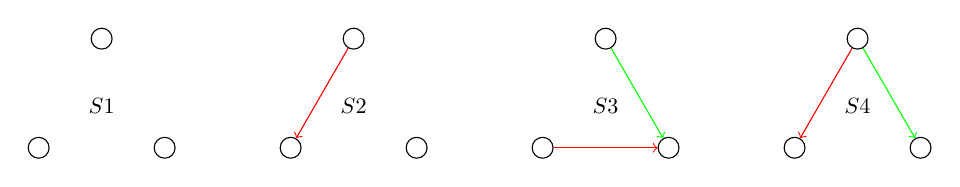
\begin{tikzpicture}[scale=0.8, every node/.style={scale=0.8}]
				
				\node (G1) at (1,0.66) {$S1$};
				\node[circle,draw] (N1) at (1,1.732) {$ $};
				\node[circle,draw] (S1) at (0,0) {$ $};
				\node[circle,draw] (C1) at (2,0) {$ $};
				
				\node (G2) at (5,0.66) {$S2$};
				\node[circle,draw] (N2) at (5,1.732) {$ $};
				\node[circle,draw] (S2) at (4,0) {$ $};
				\node[circle,draw] (C2) at (6,0) {$ $};
				
				\draw[red,->] (N2) -- (S2);
				
				\node (G3) at (9,0.66) {$S3$};
				\node[circle,draw] (N3) at (9,1.732) {$ $};
				\node[circle,draw] (S3) at (8,0) {$ $};
				\node[circle,draw] (C3) at (10,0) {$ $};
				
				\draw[green,->] (N3) -- (C3);
				\draw[red,->] (S3) -- (C3);
				
				\node (G4) at (13,0.66) {$S4$};
				\node[circle,draw] (N4) at (13,1.732) {$ $};
				\node[circle,draw] (S4) at (12,0) {$ $};
				\node[circle,draw] (C4) at (14,0) {$ $};
				
				\draw[green,->] (N4) -- (C4);
				\draw[red,->] (N4) -- (S4);
				
			\end{tikzpicture}
		\end{center}
		
		\begin{itemize}
			\item At maximum, there can only be two active fluxes.
		\end{itemize}
		
	\end{frame}
	
	%------------------------------------------------
	\section{Modeling}
	\begin{frame}
		\frametitle{Modeling of the chilean electrical network}
		
		\begin{itemize}
			\item There exists an algorithm that can find an optimal solution to Subproblem 2.
			
			\item We created a Python code that applies the algorithm to permutations to find the optimal solution for the main problem.
			
			\item This code can be iterated throughout a day to model the production plan of the whole network on a full day!
			
		\end{itemize}
	\end{frame}
	
	%------------------------------------------------
	
	
	
	\begin{frame}
		\frametitle{Demands}
		\begin{itemize}
			\item Linear interpolations with added variance that follow electricity demand curve shapes (heaps, lows, proportionality).
			\item Overall demand: \(10500[MW/h]\)
			\item North 30\%, South 10\%, Center 60\%.
		\end{itemize}
		
		\begin{figure}
			\includegraphics[width=0.63\linewidth]{Fig1_Demandas.png}
		\end{figure}
	\end{frame}
	
	%------------------------------------------------
	
	\begin{frame}
		\frametitle{Production and Technology}
		
		\begin{itemize}
			\item \(Q_N=6000[MW/h],\,Q_S=2000[MW/h],\,Q_N=12000[MW/h]\).
			\item Contributions of each type of technology to the total production on each node:
		\end{itemize}
		
		\begin{equation*}\begin{array}{c|c|c|c}
				& \text{Solar} & \text{Coal} & \text{Gas} \\ \hline
				\text{North} & 30\% & 30\% & 40\% \\
				\text{South} & 10\% & 40\% & 50\% \\
				\text{Center} & 20\% & 10\% & 70\% \\
		\end{array}\end{equation*}
	
		\begin{itemize}
			\item \(0.5\%\) energy loss on flux.
		\end{itemize}
	\end{frame}
	
	%------------------------------------------------
	
	\begin{frame}
		\frametitle{Production cost functions}
		
		\begin{itemize}
			\item Solar, Carbon and Gas cost per megawatt: 0\$, 40\$, 80\$.
			\item With technology contributions, production cost is:
		\end{itemize}
		
		\begin{equation*}\begin{aligned}
				\operatorname{p}_N(q)&=\left\{\begin{array}{cl}
					0 & ,\text{ si } 0\leq q<1800 \\
					40\cdot(q-1800) & ,\text{ si } 1800\leq q<3600 \\
					80\cdot(q-3600)+72000 & ,\text{ si } 3600\leq q\leq6000
				\end{array}\right. \\
				\operatorname{p}_S(q)&=\left\{\begin{array}{cl}
					0 & ,\text{ si } 0\leq q<200 \\
					40\cdot(q-200) & ,\text{ si } 200\leq q<1000 \\
					80\cdot(q-1000)+32000 & ,\text{ si } 1000\leq q\leq2000
				\end{array}\right. \\
				\operatorname{p}_C(q)&=\left\{\begin{array}{cl}
					0 & ,\text{ si } 0\leq q<2400 \\
					40\cdot(q-2400) & ,\text{ si } 2400\leq q<3600 \\
					80\cdot(q-3600)+48000 & ,\text{ si } 3600\leq q\leq12000
				\end{array}\right.
		\end{aligned}\end{equation*}
	\end{frame}
	
	%------------------------------------------------
	\section{Results and conclusions}
	
	\begin{frame}
		\frametitle{Results: Plots}
		
		\begin{center}
			\includegraphics[scale=0.65]{Fig2.1_Norte.png}
		\end{center}
		
	
	\end{frame}
	
	%------------------------------------------------
	
	\begin{frame}
		\frametitle{Results: Plots}
		
		\begin{center}
			\includegraphics[scale=0.65]{Fig2.2_Sur.png}
		\end{center}
		
	\end{frame}
	
	%------------------------------------------------
	
	\begin{frame}
		\frametitle{Results: Plots}
		
		\begin{center}
			\includegraphics[scale=0.65]{Fig2.3_Centro.png}
		\end{center}
		
	\end{frame}
	
	%------------------------------------------------
	
	\begin{frame}
		\frametitle{Results: Plots}
		\includegraphics[scale=0.36]{Fig2_Producciones.png}
		\includegraphics[scale=0.36]{Fig3_Flujos.png}
		
	\end{frame}
	
	%------------------------------------------------
	
	\begin{frame}
		\frametitle{Results: Plots}
		
		\begin{center}
			\includegraphics[scale=0.65]{Fig4_Funcion.png}
		\end{center}
		
	\end{frame}

	%------------------------------------------------
	
	\begin{frame}
		\frametitle{Results: Data}
		
		\begin{itemize}
			\item Total cost: 8767565.29 \$
			\item Total production: 255527.73 [MW]
			\begin{itemize}
				\item North: 79326.11 [MW]
				\item South: 25791.57 [MW]
				\item Center: 150410.05 [MW]
			\end{itemize}
			\item Total flux: 4433.55 [MW]
			\begin{itemize}
				\item North-South: 1225.3 [MW]
				\item South-North: 0.0 [MW]
				\item South-Center: 1235.01 [MW]
				\item Center-South: 0.0 [MW]
				\item North-Center: 1973.24 [MW]
				\item Center-North: 0.0 [MW]
			\end{itemize}
			\item Total energy loss: 22.17 [MW]
		\end{itemize}
		
	\end{frame}
	
	%------------------------------------------------
	
	\begin{frame}
		\frametitle{Conclusions}
		\begin{itemize}
			\item We managed to make a simple model the chilean network.
			\item The model captures trends that happen in real life (North, South and Center dynamic).
			\item Optimal solution behavior can be understood with plots.
			\item Fast to execute and apply to similar electrical networking modeling scenarios.
			
		\end{itemize}
	\end{frame}	
	
	\begin{frame}
		\frametitle{Future work ahead}
		\begin{itemize}
			\item Consider the enviromental damage of solutions.
			\item Variable productions and technology contributions.
			\item Add more nodes to the network.
			\item Non-linear cost functions.
		\end{itemize}
	\end{frame}
		
	%------------------------------------------------
	
	\begin{frame}
		\frametitle{References}
		\begin{itemize}
			\item Universidad de Chile, Facultad de Ciencias F\'isicas y Matem\'aticas, Mariano Vazquez, Estudio de Problemas de Optimizaci\'on y Equilibrio sobre una Red de Producci\'on El\'ectrica, 2023.
			\item Comisión Nacional de Energía - Reporte Energético Financiero - Vol. Nº10 - 2019.
			\item U.S. Energy Information Administration, Demand for electricity changes through the day, APRIL 6, 2011.
			\item  © 2023 Society for Industrial and Applied Mathematics, Pollution Regulation for Electricity Generators in a Transmission Network, Nicol\'as Hern\'andez-Santib\'a\~{n}ez, Alejandro Jofr\'e and Dylan Posamma.	
		\end{itemize}
	\end{frame}
	
	\begin{frame}[plain] % The optional argument 'plain' hides the headline and footline
		\begin{center}
			{\LARGE Thank you for your attention :)}
			
			\bigskip\bigskip % Vertical whitespace
			
			{\LARGE Questions? Comments?}
		\end{center}
	\end{frame}
	
	%----------------------------------------------------------------------------------------
	
\end{document} 